\documentclass{ctexart}
\usepackage{amsmath,bm}
\usepackage{setspace}
\usepackage{xeCJK}
\usepackage{indentfirst}
\usepackage{listings}
\usepackage{graphicx}
\usepackage{subfigure}
\usepackage{amsfonts,amssymb}
\usepackage[a4paper,scale=0.8]{geometry}
\usepackage{hyperref}
\setCJKmainfont{华光书宋_CNKI}
\newCJKfontfamily\kaiti{华光楷体_CNKI}
\newCJKfontfamily\hei{华光黑体_CNKI}
\newCJKfontfamily\fsong{华光仿宋_CNKI}
\newfontfamily\code{Courier New}
\linespread{1.5} \setlength\parindent{2 em}
\title{\Huge 中国科学技术大学计算机学院\\《计算机图形学理论和应用》调研报告}
\date{\LARGE 2021.05.26}
\begin{document}
\begin{hei}  \maketitle\end{hei}
\begin{figure}[htbp]	
	\centering	
	
\includegraphics[scale=0.4]{USTC.png}
		
\end{figure}
\begin{LARGE}\begin{align*}&\text{调研题目:\underline{人脸动画及表情合成技术发展综述}}\\ 
	&\text{学生姓名:\underline{胡毅翔}}\\
	&\text{学生学号:\underline{PB18000290}}\end{align*}\end{LARGE}
 \par 
 \par\par
\centerline{\large 计算机实验教学中心制}
\par \centerline {\large 2019年9月}
\newpage
\tableofcontents
\newpage
\section{\hei 引言}
具有真实感的人脸脸表情动画合成一直是计算机图形学和计算机视觉领域的研究热点和难点之一,且被广泛应用于数字娱乐、视频会议、医疗、辅助教育等领域。在人脸动画领域,高端方法和低端方法之间存在很大的差距。高端方法生成的面部动画令真正的人类难以区分,但是需要人脸建模的专家付出大量的体力劳动。而低端方法,依托传感器的面部捕捉等,得到人脸动画参数,生成人类动画,又不足以表现人脸自然变化中的细节。为此,研究者们不断钻研,在鲁棒性,性能,易用性,实时性等方面得到了优化。\par
目前,人脸表情合成方法主要分为三大类:基于几何模型(三维网格模型)的人脸表情合成,基于二维图像的人脸表情合成和基于深度神经网络的人脸表情合成。随着应用场景不断拓宽,人脸表情动画的驱动方式也不断增加,从最初的参数驱动,到图像数据驱动,再到音频,文本驱动。\par
\section{\hei 基于几何模型}
基于三维网格的方法是通过跟踪一系列人脸表情变化的曲线和基于全局统计的模型生成所需的目标图像。\par
\subsection{\hei 整体法}
基于这种传统方法,有以下这些主要成果:Pighin等\cite{1}提出了具有逼真纹理的三维人脸建模的表情合成系统。
Wang等\cite{2}构建了一个MPEG-4兼容的人脸动画系统,使用脸部定义参数( facial definition parameter, FDP)来构建人脸模型,通过脸部动画参数( facial animation parameter, FAP)来驱动该模型生成各种表情。
Blanz等\cite{3}提出了从单张图片或视频中恢复人脸的三维模型,尝试从带纹理的三维模型中进行表情合成,但创建一个好的模型相当困难,因为必须对面部的所有细节进行建模,如眼睛、头发、牙齿等。
Vlasic等\cite{4}提出的多线性模型(Multilinear Models)将分离参数化不同的属性(如顶点信息、形状、视位、表情等)建立在同一个数据张量空间中, 这些属性之间用笛卡尔积来构造并且相互独立。将这些独立属性参数进行任意组合,最终得到不同的人脸表情。
Lv等\cite{5}提出一种面向同一人脸表情转移的方法,即对目标人脸进行三维建模,生成特定的混合形状(blendshape)模型,利用该模型生成与输入人脸图像匹配的三维人脸模型,并对图像进行扭曲融合,生成所需的目标人脸图像。
\par
\begin{figure}[htbp]	
	\centering	
	\subfigure[1.1]{
		\begin{minipage}[t]{0.5\linewidth}
			\centering
			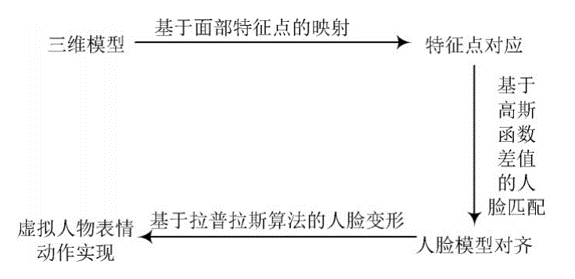
\includegraphics[scale=0.5]{1.png}
			%\caption{fig1}
		\end{minipage}%
	}%
	\subfigure[1.2]{
		\begin{minipage}[t]{0.5\linewidth}
			\centering				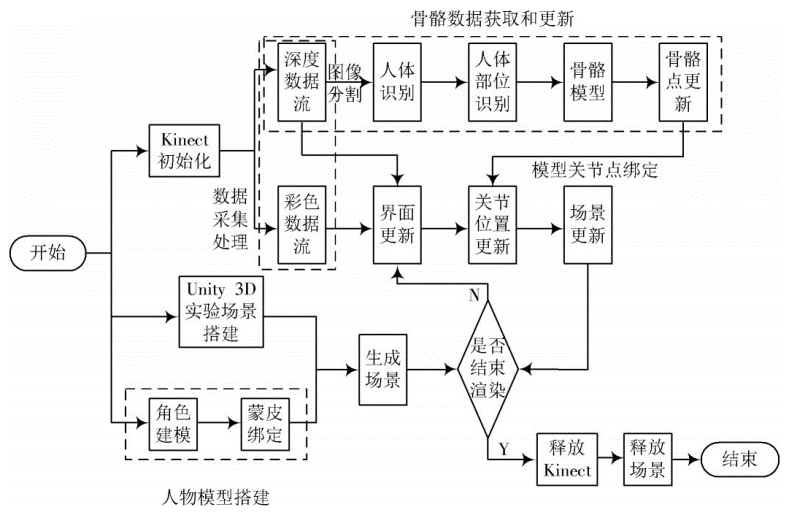
\includegraphics[scale=0.5]{2.png}
			%\caption{fig2}
		\end{minipage}%
	}
	\caption{虚拟人物表情动作系统}
\end{figure}
Xiong等\cite{23}基于几何模型构建了一个虚拟人物表情动作系统,利用系统硬件模块完成图
像数据及人体骨骼数据的采集、处理,以及人体骨骼点定位、关节点与 Kinect 骨骼点映射关系构建、虚拟人物模型的搭建。
在此基础上,通过面部特征点映射完成特征点的对应,并通过对齐视频人脸与三维动画虚拟人脸,完成人脸模型对齐;采用
拉普拉斯坐标恢复模型重建人脸表情动作,完成三维动画虚拟人物表情动作的模拟,实现基于三维动画的虚拟人物表情动
作系统设计。

\subsection{\hei 分治法}
尽管上述整体法较为稳定,且便于计算,但这些方法通常不允许细粒度变形,并且在困难区域(嘴巴,眼睛)难以生成逼真的效果。而人们往往是通过这些五官特征来区分人脸的。为了解决五官特征不明显,不真实的问题,人们又基于分而治之的思想,提出了对五官,皱纹等细节部位先进行单独处理,再通过一定的约束合成人脸模型,以提高人脸的真实感。\par
Pasquariello等\cite{6}在三维人脸模型 中加入皱纹等细节因素,将人脸模型进行网格化,并按照人的生理结构将人脸分成嘴、眼睛、眉毛、额头等区域,使得每一区域的网格数量和拓扑等都不同,进而实现表情的模拟。\par
\begin{figure}[htbp]	
	\centering	
	\subfigure[2.1]{
		\begin{minipage}[t]{0.3\linewidth}
			\centering
			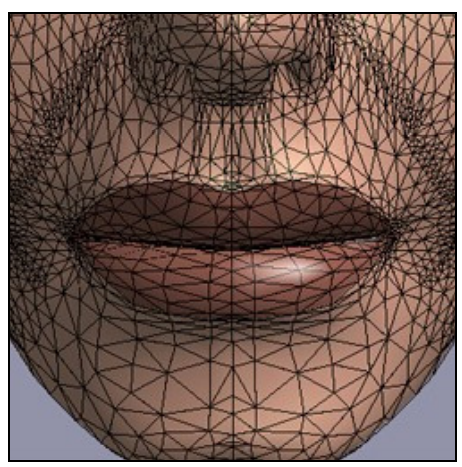
\includegraphics[scale=0.3]{3.png}
			%\caption{嘴}
		\end{minipage}%
	}%
	\subfigure[2.2]{
		\begin{minipage}[t]{0.3\linewidth}
			\centering				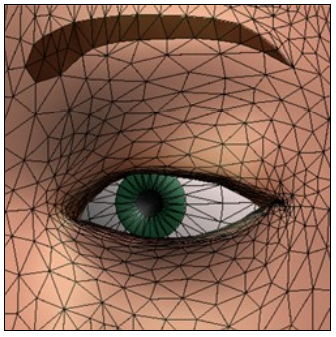
\includegraphics[scale=0.3]{4.png}
			%\caption{眼睛}
		\end{minipage}%
	}
	\subfigure[2.3]{
		\begin{minipage}[t]{0.3\linewidth}
			\centering				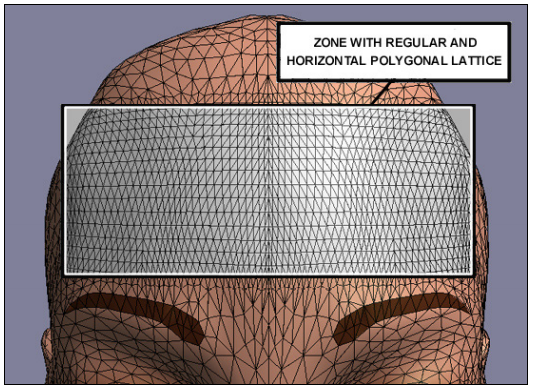
\includegraphics[scale=0.3]{5.png}
			%\caption{额头}
		\end{minipage}%
	}
	\caption{分治法}
\end{figure}
Zhang等\cite{7}在三维形变模型中也加入了皱纹等细节,将其划分为14个子区域,避免了表情皱纹超过分区的边界。
Joshi等\cite{8}提出的基于物理的分割方法可以自动将人脸分割成多个区域,每一个区域都表示成混合形状的线性组合,从混合形状中学习约束条件和参数。
Park等\cite{9}将给定的每一个源关键模型分成3个子区域,每一个子区域都包含人脸的关键特征,实现了面部表情的合成。
Joshi\cite{10}把每一个表情看成 其他表情的线性组合,通过改变这些线性组合的权重来合成比较完整的面部表情。
Garrido\cite{11}提出了一种基于图像的人脸视频再现方法,对于输入的两个不同人脸的面部表情视频, 将源序列的表情传递给目标序列,同时尽可能地保留灯光、背景等因素。该方法的缺点是:需要一些特定的人脸数据库,且依赖于输入图像的一些表情信息,如是否是中性人脸或者有无标记点等等。
文献\cite{12,13}首先对人脸进行建模,然后得到特定用户的混合形状模型,进而求解出混合形状系数, 最后通过对系数的改变来合成目标表情。
Huang等\cite{14}提出了基于非联合学习的人脸表情合成方法:通过一种无监督回归的算法,将具有相同属性的三维人脸模型映射到同一个低维空间,对其进行重建,实现人脸表情的合成。
\section{\hei 基于二维图像}
基于二维图像的方法是用已知的表情数据来合成新的表情,或者直接将已有的表情传递到目标图像上。
\subsection{\hei 表情映射法}
Williams\cite{15}提出通过表情映射的方法来合成新的目标表情,首先提取两幅图像不同的面部特征,然后计算特征之间的矢量差, 最后利用特征向量来进行图像的扭曲。该方法的鲁棒性不足,虽然实现了不同表情之间的转换,但是不适用于戴眼镜和头部位姿有较大变化的情况。
\subsection{\hei 表情流法}
Yang等\cite{16}提出了基于表情流的方法:首先提取两幅图像的特征点并分别进行三维人脸重建;然后计算两个三维模型之间的差异,将差异映射到二维图像上得到表情流,再利用所得表情流进行图像扭曲;最后进行图像融合\cite{17}。 
\begin{figure}[htbp]	
	\centering	
	
			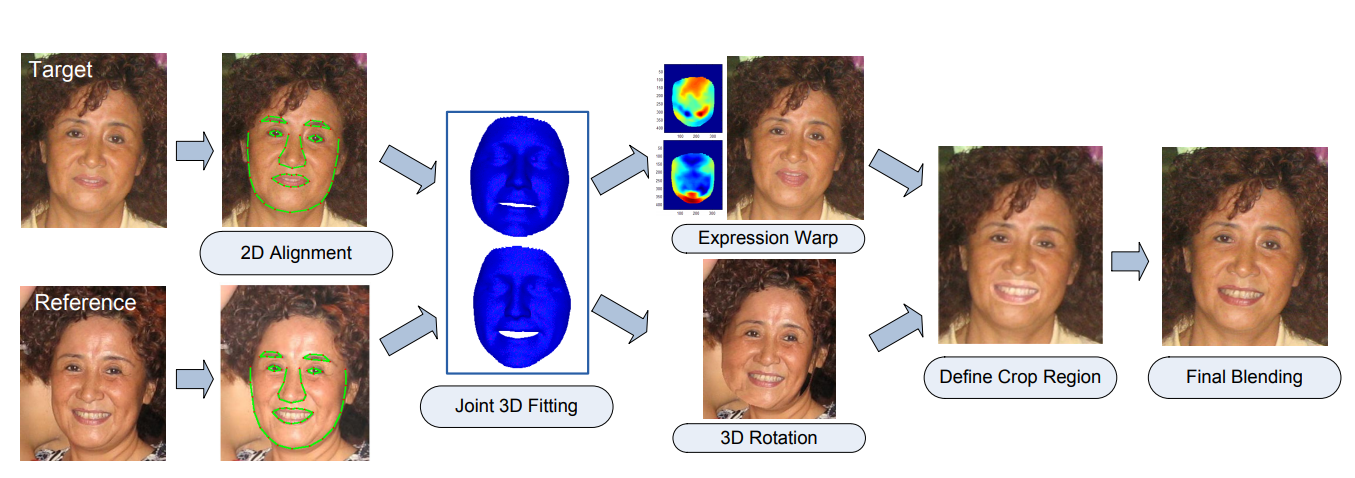
\includegraphics[scale=0.3]{6.png}
	\caption{表情流法}
\end{figure}
\subsection{\hei 替换法}
表情流的计算方法往往比较复杂,鲁棒性很差,得到的效果不是很逼真,而且只能在同一人脸之间进行,不具有普遍性。文献\cite{18,19}提出了一种人脸图像自动替换系统:首先对输入图 像进行人脸检测;然后将提取的每个人脸进行对齐,并从大量的人脸数据库中找到与其相近的人脸;最后通过图像融合实现目标输入图像的表情合成。这些方法可以有效、快捷地合成人脸表情,但由于人脸具有特异性,且表情复杂、丰富,在表情合成过程中合成具有真实感的表情比较困难。
\begin{figure}[htbp]	
	\centering	
	
			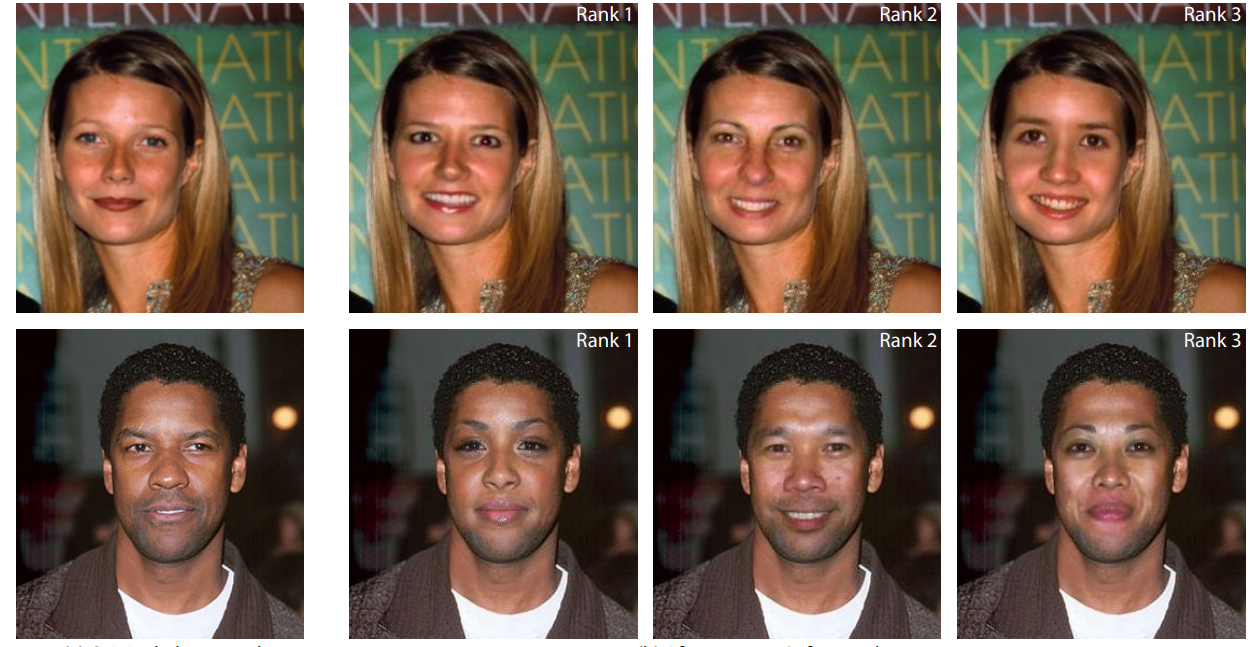
\includegraphics[scale=0.3]{7.png}
	\caption{替换法}
\end{figure}
\section{\hei 基于深度神经网络}
基于深度神经网络的方法是在上述两种方法的基础上,结合深度神经网络,提供一种端到端的人脸表情生成方法。这些方法相较传统方法在实时性,鲁棒性等方面有所提高。\par
\subsection{\hei FLAME模型}
Li等\cite{20}提出了FLAME(Faces Learned with an Articulated Model and Expressions)模型,通过从数千个精确对齐的3D扫描中学习人脸模型。该模型以下巴,脖子,眼球,姿态相关校正等线性组合而成,模块化处理,可以对各个部分进行精细化处理,并且最终得到的是低维表示。\par
\begin{figure}[htbp]	
	\centering	
	
			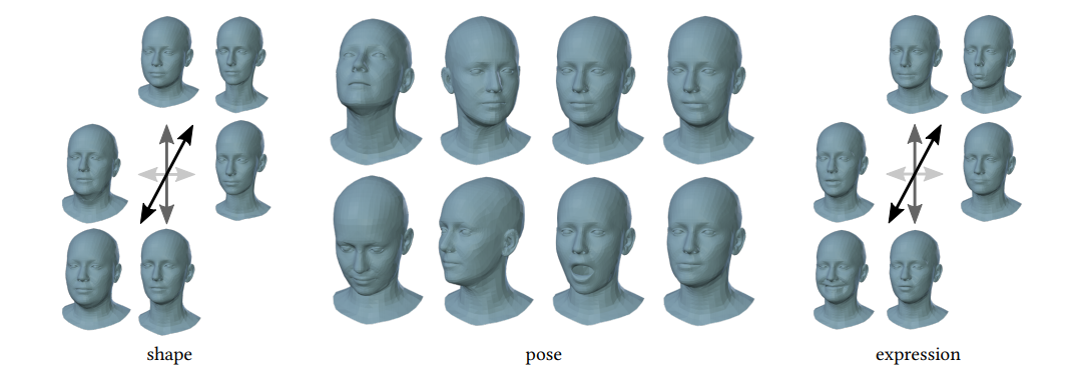
\includegraphics[scale=0.5]{8.png}
	\caption{FLAME模型}
\end{figure}
Sanyal等\cite{21}在FLAME模型的基础上假设脸部形状是恒定的,与表情,状态,光线等无关,实现了从单张2D图像得到FLAME模型的神经网络。这种方法进一步摆脱了对3D扫描的依赖,是一种无3D监督的学习,使得模型构建更为简便,还维持了很好的鲁棒性。\par
Paier等\cite{22}提出了一种混合动画空间,该框架利用深度学习来提供一个交互式动画引擎,可以提供简单直观的可视化将其用于面部表情编辑。此外,该框架还训练了这个变分式自动编码器,以学习用于交互式面部动画的人脸表情的低维潜在空间。
\par
\subsection{\hei 音频驱动}
Hai\cite{Hai}等提供了一个用原始波形进行实时语音驱动生成3D人脸动画的深度学习框架。该网络直接映射输入语音序列到一系列面部动作单元激活和头部旋转用以驱动3D混合形状人脸模型。该模型还能学习语音的上下文中的潜在情感变化,使得人脸动画的情绪强度与语音的情绪强度相当。
\par
Cudeiro\cite{Cudeiro}等则提供了一个鲁棒性更强的深度神经网络。该网络同样由音频驱动,输入为任何语言和一个人脸模型,而输出为一段连续的人脸动画。
\begin{figure}[htbp]	
	\centering	
	
			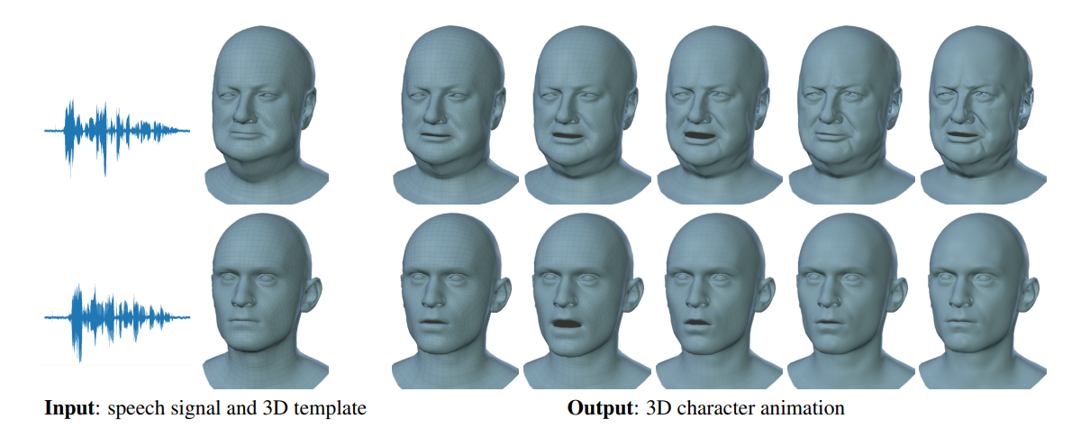
\includegraphics[scale=0.7]{9.png}
	\caption{音频驱动}
\end{figure}
\subsection{\hei 文本驱动}
给定文本作为输入时,Yu等\cite{Yu}提供了采用深度学习方法合成高真实感、认以身份以及唇音同步的人类动画。

\section{\hei 总结}
人脸动画表情技术的发展经历了从早期的几何模型生成,到基于二维图像生成,再到混合使用几何模型及二维图像,结合音频,文本输入,构建端到端神经网络。人脸的真实感不断增强,计算效率不断提高,算法的鲁棒性,实时性,可用性不断增强。随着技术的不断完善,人们对数字人的接受程度也越来越高,人脸动画在VR,AR,游戏,CG电影等领域得到了广泛应用。\par
在未来的研究过程中,基于深度神经网络的生成方法将成为主流,设计更为简单易用的,对计算性能需求更低的算法,使得个人用户可以在PC甚至移动设备端实现人脸动画的生成。同时,对于细节(眼部,脸部,鼻子等)的处理也更加真实。\par
此外,目前的研究中生成的人脸模型,以单纯的表面效果为主。未来的研究中,为使人脸更加真实,对口腔,鼻腔等原本被忽略的可视脸部器官模型也需要进一步完善。
\begin{thebibliography}{99}
	\bibitem{1} Frédéric Pighin, Jamie Hecker, Dani Lischinski, Richard Szeliski, and David H. Salesin. 1998. Synthesizing realistic facial expressions from photographs. In Proceedings of the 25th annual conference on Computer graphics and interactive techniques (SIGGRAPH '98). Association for Computing Machinery, New York, NY, USA, 75–84.
	\bibitem{2} 王奎武,王洵,董兰芳,陈意云.一个MPEG-4兼容的人脸动画系统[J].计算机研究与发展,2001(05):529-535.
	\bibitem{3}Blanz, V. and Basso, C. and Poggio, T. and Vetter, T.Reanimating Faces in Images and Video.Computer Graphics Forum
	\bibitem{4}Daniel Vlasic, Matthew Brand, Hanspeter Pfister, and Jovan Popović. 2005. Face transfer with multilinear models. ACM Trans. Graph. 24, 3 (July 2005), 426–433. 
	\bibitem{5}LV P, XU M L. Expression of Face Expressions Unrelated to
Expression Database $[\mathrm{J}] .$ Journal of Computer-Aided Design \&
Computer Graphics, $2016,28(1)$.
\bibitem{23}熊伟.基于三维动画的虚拟人物表情动作系统设计[J].现代电子技术,2020,43(20):97-101.

\bibitem{6}PASQUARIELLO S, PELACHAUD C. GRETA: A Simple Facial Animation Engine[M]// Soft Computing and Industry. London ; Springer, 2002 .
\bibitem{7}ZHANG Q,LIU Z,GUO B, et al. Geometry-Driven Photorealistic Facial Expression Synthesis $[\mathrm{J}] .$ IEEE Transactions on Visualization \& Computer Graphics, $2005,12(1): 48-60 .$
\bibitem{8}
JOSHI P, TIEN W C,DESBRUN M, et al. Learning controls for
blendshape based realistic facial animation $[\mathrm{C}] / /$ Proceedings of
ACM SIGGRAPH Eurographics Symposium on Computer Aimation. $2003: 187-192 .$
\bibitem{9}PARK B, CHUNG H, NISHITA T, et al. A feature-based approach to facial expression cloning: Virtual Humans and Social
Agents [J]. Computer Animation and Virtual Worlds, 2005 ,
$16(3 / 4): 291-303 .$
\bibitem{10}JOSHI P, TIEN W C, DESBRUN M, et al. Learing Cnotrols for
Blend Shape Based Realistic Facial Animation [ $\mathrm{C}$ ]// ACM
Transactions on Graphics. $2006.426-433 .$
GARRIDO P, VALGAERTS L, REHMSEN O, et al. Automatic
face reenactment
\bibitem{11}
Proceedings of IEEE Conference on Computer Vision and Pattern Recognition. Los Alamitos: IEEE Computer Society Press, 2014:4217-4224.
\bibitem{12}
WESIE T, BOUAZIZ S,LI H, et al. Realtime performance-based
facial animation $[\mathrm{J}]$. ACM Transactions on Graphics, 2011 ,
$30(4): 1 .$
\bibitem{13}
CAO C, WENG Y, LIN S, et al. 3D shape regression for real-
time facial animation[J]. ACM Transactions on Graphics, 2013 ,
$32(4): 1 .$
\bibitem{14}
HUANG X Q, LIN Y X, SONG M L. Three-dimensional facial
expression synthesis method based on nonlinear joint learning
Journal of Computer-Aided Design \&. Computer Graphics, $2011 , 23(2).$
\bibitem{15}WILLIAMS L. Performance-driven facial animation $[\mathrm{C}] / / \mathrm{ACM}$
SIGGRAPH Computer Graphics. $1990: 235-242 .$
\bibitem{16}
YANG F, WANG J, SHECHTMANE, et al. Expression flow for
3D-aware face component transfer [ J]. ACM Transactions on
Graphics, $2011,30(4): 1$.
\bibitem{17}
PEREZ P,GANGNET M,BLAKE A. Poisson image editing
$[\mathrm{J}]$. ACM Transactions on Graphics, $2003,22(3): 313-318$.
\bibitem{18}
BITOUK D. Face Swapping : Automatically Replacing Faces in
Photographs $[\mathrm{J}] .$ ACM SIGGRAPH, $2008,27(3): 1-8$.
\bibitem{19}
DALE K, SUNKAVALLI K, JOHNSON M $\mathrm{K}$, et al. Video face
replacement $[\mathrm{J}] .$ ACM Transactions on Graphics, $2011,30(6): 1 .$
\bibitem{20}
Tianye Li,Timo Bolkart,Michael J. Black,Hao Li,Javier Romero. Learning a model of facial shape and expression from 4D scans[J]. ACM Transactions on Graphics (TOG),2017,36(6).
\bibitem{21}
Soubhik Sanyal, Timo Bolkart, Haiwen Feng, Michael J. Black. Learning to Regress 3D Face Shape and Expression From an Image Without 3D Supervision. In IEEE Conference on Computer Vision and Pattern Recognition, CVPR 2019, Long Beach, CA, USA, June 16-20, 2019. pages 7763-7772, Computer Vision Foundation / IEEE, 2019.
\bibitem{22}
Paier Wolfgang,Hilsmann Anna,Eisert Peter. Interactive facial animation with deep neural networks[J]. IET Computer Vision,2020,14(6).

\bibitem{Hai}
Hai Xuan Pham,Yuting Wang,Vladimir Pavlovic. End-to-end Learning for 3D Facial Animation from Speech[P]. Multimodal Interaction,2018.
\bibitem{Cudeiro}
Cudeiro D, Bolkart T, Laidlaw C, et al. Capture, learning, and synthesis of 3D speaking styles[C]//Proceedings of the IEEE/CVF Conference on Computer Vision and Pattern Recognition. 2019: 10101-10111.

\bibitem{Yu}
于灵云. 基于文本/语音驱动的高自然度人脸动画生成[D].中国科学技术大学,2020.
\end{thebibliography}
\end{document}